\documentclass[10pt,oneside]{estiloUBI}
\include{formatacaoUBI}

%\usepackage[english,portuges]{babel}
%\usepackage[utf8]{inputenc}
%\usepackage[T1]{fontenc}
\usepackage{siunitx}
%\usepackage{graphicx}
\usepackage{minted}
\usepackage{tikz}
\usepackage{pgfplots}
%\usepackage{hyperref}
\usepackage[printonlyused]{acronym}

%\graphicspath{{img/}}

\pgfplotsset{compat = newest}

\newcommand{\chronOS}{\textsf{chronOS}}
\newcommand{\git}{\textsf{git}}

%\title{
%	Sistemas Operativos --- Projeto\\
%	\chronOS~--- \textbf{Relatório final}
%}
%
%\author{
%	\begin{tabular}[!h]{l l}
%		39489 & Jorge Miguel Louro Pissarra\\
%		41266 & Diogo Castanheira Simões\\
%		41381 & Igor Cordeiro Bordalo Nunes
%	\end{tabular}
%}
%
%\date{\today}

\portugues
\makeindex

\cabecalho{\chronOS~1.2.0}

\begin{document}
	\onehalfspacing
	\pagenumbering{roman}
	\begin{titlepage}
\begin{center}

\begin{flushleft}
\includegraphics[height=2.22cm]{logo}\\
\rostoubi UNIVERSIDADE DA BEIRA INTERIOR\\
\rostofac Departamento de Informática\\
\end{flushleft}

%\vspace{7.6cm}
\vspace{1.5cm}

\begin{center}
\includegraphics[height=5cm]{chronos.png}
\end{center}

\rostotitulo \textbf{\chronOS~\version} \\
\rostosubtit \textit{A scheduling simulator}\\

\vspace{1.8cm}

\begin{tabular}{>{\rostonomes\bfseries}l @{\rostonomes\bfseries~---~} >{\rostonomes\bfseries}l}
	39489 & Jorge Miguel Louro Pissarra \\
	41266 & Diogo Castanheira Simões \\
	41381 & Igor Cordeiro Bordalo Nunes \\
\end{tabular}

\vspace{1.4cm}

\rostooutros Sistemas Operativos\\
\rostonomes \textbf{Engenharia Informática}\\
\rostooutros (1º ciclo de estudos)\\

\vspace{2.1cm}

\rostooutros Docente: Prof. Doutor Paul Andrew Crocker\\
% \rostooutros Orientador: Prof. Doutor João Paulo da Costa Cordeiro\\
%Co-orientador: Prof. Doutor Nome\\

\vspace{1.2cm}

\rostooutros \textbf{Covilhã, 14 de junho de 2020}

\end{center}
\end{titlepage}


	
	%\dominitoc
	
	\pagestyle{fancy}
	
	%\cleardoublepage
	\newpage
	
	\section*{\titulos{Resumo}}
	\vspace{0.5cm}
	
	\chronOS~é um programa de simulação de escalonamento de processos e gestão de memória.
	
	Encontra-se implementado o algoritmo FCFS para o escalonamento, assim como o algoritmo \textit{first-fit} para a gestão de memória estática.
	
	Um gestor de memória dinâmica (\textit{heap memory}) foi implementado recorrendo a listas ligadas. Quatro algoritmos foram utilizados para fazer a respetiva gestão. Para cada algoritmo foi criada uma memória dedicada para fins estatísticos e comparativos.
	
	Um plano de execução é lido no arranque do programa e o simulador de CPU, definido para \SI{2}{\hertz}, invoca o método que implementa o algoritmo de escalonamento para decidir a próxima ação, a qual pode ser um \textit{switch} no estado de um processo ou a execução de uma instrução.
	
	Sempre que possível é utilizada a memória \textit{heap} do computador para albergar os componentes do programa. Tal inclui o bloco de memória estática, a tabela PCB e as quatro memórias dinâmicas.
	
	No presente relatório é apresentada a versão 1.2.0.

	
	%\cleardoublepage
	\tableofcontents
	\listoffigures
	%\cleardoublepage	
	\mainmatter


	
	\chapter{Pesquisa e desenvolvimento}
	\label{sec:dev}
	
	Conhecer o coração dos sistemas operativos modernos implica conhecer diversos métodos de gestão de memória e de processos. \chronOS~propõe-se enquanto projeto de simulação de escalonamento a fim de consolidar conhecimentos na área no âmbito da unidade curricular de Sistemas Operativos.
	
	\section{Linguagem e pesquisa}
	\label{ssec:dev:sota}
	
	Para este projeto foram consideradas as linguagens C, C++ e OCaml. Optou-se pela linguagem C devido à facilidade em se trabalhar a um mais baixo nível e à grande versatilidade que os apontadores permitem. C++ teria sido uma linguagem ideal para usar orientação a objetos, mas a pouca familiaridade com esta forçou-nos a optar pelo C.
	
	Para reforçar a nossa aprendizagem, decidimos implementar tudo \textit{in-house}, \textbf{não} recorrendo a códigos já existentes ou projetos semelhantes na Internet e em repositórios \git~públicos.
	
	
	\section{Repositório no GitLab}
	\label{ssec:dev:gitlab}
	
	O projeto encontra-se alojado num servidor GitLab privado no seguinte \textit{link}: \url{https://gitlab.pcdev.pt/inunes/chronos/}
	
	O repositório \git~em causa inclui vários \textit{branches} nos quais nos encontramos a trabalhar, a saber:
	
	\begin{itemize}
		\item \texttt{master}: \textit{branch} principal para onde é feito \textit{merge} de versões finais funcionais;
		\item \texttt{dev}: \textit{branch} de desevolvimento dedicado do elemento de grupo Jorge Pissarra;
		\item \texttt{dev-in}: \textit{branch} de desevolvimento dedicado do elemento de grupo Igor Nunes (regra geral é neste \textit{branch} que se encontram as \textbf{versões compiláveis sem erros com recurso ao \texttt{Makefile}});
		\item \texttt{dev-ds}: \textit{branch} de desevolvimento dedicado do elemento de grupo Diogo Simões;
	\end{itemize}
	

	\section{Resumo do projeto}
	\label{ssec:dev:summary}
	
	À data de escrita do presente relatório, o programa \chronOS~é capaz de fazer as seguintes tarefas:
	
	\begin{enumerate}
		\item Alocar células de memória e a tabela \texttt{\ac{PCB}};
		\item Alocar 4 memórias \textit{heap} (uma por algoritmo de gestão);
		\item Ler o ficheiro \texttt{plan.txt} e guardar em memória o plano de execução numa \textit{queue};
		\item Temporizar o sistema de 500 em 500 milissegundos;
		\item Extrair de um ficheiro \texttt{*.prg} as suas instruções;
		\item Alocar em memória as instruções referentes a um programa recorrendo ao \textbf{algoritmo \textit{first-fit}};
		\item Ler um programa para memória e alocar os dados na tabela \ac{PCB} ao tempo exato indicado pelo plano de execução;
		\item Executar as instruções em memória, incluindo o \textit{fork} (instrução \verb|C n|) e o \textit{clean} (instrução \verb|L filename|);
		\item Gerir os processos com recurso ao \textbf{algoritmo \ac{FCFS}};
		\item Alocar e dealocar memória \textit{heap} a pedido de cada processo;
		\item Alocar memória \textit{heap} por solicitação aleatória do processo principal;
		\item Imprimir um relatório do estado dos processos;
		\item Imprimir um relatório do estado da memória em modo \textit{debug};
		\item Imprimir um relatório das memórias \textit{heap};
		\item Fazer um \textit{dump} das memórias \textit{heap} em modo \textit{debug};
		\item Libertar os recursos associados às memórias, à tabela \ac{PCB} e à \textit{queue} do plano de execução.
	\end{enumerate}
	
	Todas as tarefas foram testadas em modo \textit{debug} recorrendo a \textit{sanitizer flags} (descritas na secção \ref{ssec:dev:struct_makefile}) que nos permite verificar que não existe nenhum \textit{memory leak} no final da execução do programa.
	
	
	\section{Estrutura do código e \texttt{Makefile}}
	\label{ssec:dev:struct_makefile}
	
	A pasta de desenvolvimento está estruturada com as seguintes pastas:
	
	\begin{itemize}
		\item \verb|doc|: pasta onde é escrita a documentação, incluindo este mesmo documento em \LaTeX;
		\item \verb|include|: inclui todos os \textit{header files} (ficheiros \verb|*.h|) necessários ao programa;
		\item \verb|src|: inclui todos os ficheiros \verb|*.c| com a implementação dos protótipos declarados nos \textit{header files}.
	\end{itemize}
	
	Por sua vez, o \texttt{Makefile} está construído de forma a possibilitar 2 formas de compilação:
	
	\begin{itemize}
		\item \textbf{\textit{Debug}} (\verb|make debug|): versão de desenvolvimento com mensagens de \textit{debugging} bastante detalhadas;
		
		\item \textbf{\textit{Release}} (\verb|make release|): versão final sem mensagens de \textit{debug} durante a execução do \chronOS.
	\end{itemize}

	O \texttt{Makefile} inclui uma série de \textit{flags} adicionais face ao comum a fim de controlar de forma mais apertada o comportamento do \ac{GCC}, o qual é bastante permissivo por natureza. O modo \textit{debug} inclui \textit{sanitizer flags} que permitem detetar \textit{memory leaks} e detalhar informações acerca de falhas graves na execução relacionadas com acessos indevidos à memória (os clássicos \textit{segmentation faults}).
	
	
	\chapter{Execução do \chronOS}
	\label{sec:main}
	
	O programa começa por alocar todos os recursos necessários à execução do programa, nomeadamente:
	
	\begin{itemize}
		\item \verb|memory|: bloco de memória, descrito na secção \ref{sec:memory}, constituída por 1000 células;
		\item \verb|pcb|: tabela \ac{PCB}, descrita na secção \ref{sec:process}, constituída por 100 linhas;
		\item \verb|plan|: \textit{queue} com o plano de entrada de processos no sistema, dinamicamente alocada e ajustada;
		\item \verb|heap_*|: memórias \textit{heap}, constituídas por 128 partições de 2 KB cada, uma por cada algoritmo de gestão implementado, a saber:
		\begin{enumerate}
			\item \verb|heap_first|: reservada para o algoritmo \textit{first-fit};
			\item \verb|heap_next|: reservada para o algoritmo \textit{next-fit};
			\item \verb|heap_best|: reservada para o algoritmo \textit{best-fit};
			\item \verb|heap_worst|: reservada para o algoritmo \textit{worst-fit}.
		\end{enumerate}
	\end{itemize}

	O plano de entrada de processos é lido a partir do ficheiro \texttt{plan.txt}, o qual deve estar obrigatoriamente presente. O plano é alocado em \textit{heap memory} numa \textit{queue} do tipo \verb|plan_q|, definida em \verb|plan.h|. É esperado que o ficheiro tenha os dados ordenados por ordem cronológica de entrada. O comportamento do \chronOS~ para um plano não ordenado não está definido.
	
	\chronOS~executa com base num ciclo que simula uma \ac{CPU} com um \textit{clock} de \SI{2}{\hertz}. A cada ciclo de \textit{clock} é considerado que passou 1 unidade de tempo de \ac{CPU}, armazenada em \verb|cputime|, e que permite determinar os tempos aos quais os processos entram em execução, quanto tempo levam a ser executados e em que tempo são terminados.
	
	A cada ciclo de \textit{clock}, um algoritmo de escalonamento é executado, o qual irá definir a próxima ação a ser tomada. Os algoritmos de escalonamento têm o controlo \textit{de facto} da execução das instruções e dos processos, não sendo responsabilidade da função \verb|main| onde se encontra o simulador da \ac{CPU}.
	
	\begin{figure}[!btp]
		\centering
		\includegraphics[width=\textwidth]{pcbreport}
		\caption{Exemplo de um relatório da tabela de processos.}
		\label{fig:pcbreport}
	\end{figure}
	
	\begin{figure}[!btp]
		\centering
		\includegraphics[scale=0.6]{memreport}
		\caption{Exemplo de um relatório da memória estática em modo \textit{debug}.}
		\label{fig:memreport}
	\end{figure}

	Também é determinado por um método aleatório se o processo principal do \chronOS~deverá alocar memória dinâmica e, em caso positivo, quantos blocos deverão ser alocados, entre o mínimo e o máximo permitidos (i.e., entre 3 e 10). Este processo será explorado em mais detalhe na Secção \ref{sec:heap}, assim como os algoritmos de gestão de memória implementados.

	Para terminar, todos os recursos são libertados e é impresso um relatório da tabela \ac{PCB} (Figura \ref{fig:pcbreport}) e um das memórias dinâmicas (Figura \ref{fig:heapreport}). Em modo de \textit{debug}, e exclusivamente para efeitos de \textit{debugging} no processo de desenvolvimento, é impresso um relatório adicional da memória estática (Figura \ref{fig:memreport}) e \textit{dumps} das 4 memórias dinâmicas (Figura \ref{fig:heapdump}).
	
	
	\section{Argumentos passados pela linha de comandos}
	\label{ssec:main:argv}
	
	\chronOS~admite passagem opcional de argumentos pela linha de comandos a fim de modificar a configuração padrão do programa, definida com a estrutura \mintinline{c}{struct world w} (definida em \verb|types.h|, declarada em \verb|data.h| e inicializada em \verb|world.c|).
	
	A sintaxe é a seguinte:
	
	\begin{verbatim}
./chronos
   [<--fcfs | --sjf | <--rr | --robin | --round-robin>>]
   [<--seed | -s> n]
	\end{verbatim}
	
	\begin{enumerate}
		\item Definição do algoritmo de escalonamento:
		\begin{itemize}
			\item \verb|--fcfs|: algoritmo \ac{FCFS} (algoritmo definido por defeito);
			\item \verb|--sjf|: algoritmo \ac{SJF};
			\item \verb|--rr|, \verb|--robin| ou \verb|--round-robin|: algoritmo \textit{round-robin}. 
		\end{itemize}
	
		\item Definição da semente de solicitações pseudoaleatórias da memória \textit{heap}:
		\begin{itemize}
			\item \verb|--seed n| ou \verb|-s n|: define semente dada pelo número inteiro \verb|n|. Caso seja fornecido um número fraccionário é admitida a parte inteira. Em caso de não ser um número é definido 0 (zero). O valor por defeito é definido pelo tempo (descrito na secção \ref{ssec:heap:request}).
		\end{itemize}
	\end{enumerate}
	
	Chamadas válidas do \chronOS~incluem:
	
	\begin{verbatim}
./chronos
./chronos --seed 2020
./chronos --fcfs -s 15
	\end{verbatim}
	
	
	
	\chapter{Gestão de processos}
	\label{sec:process}
	
	Um \textbf{processo} inclui as seguintes informações, definidas na estrutura \verb|process| no \textit{header file} \texttt{types.h}:
	
	\begin{itemize}
		\item \verb|name|: nome do processo;
		\item \verb|pid|: \ac{PID} do processo;
		\item \verb|ppid|: \ac{PID} do processo pai;
		\item \verb|context|: variável inteira associada ao processo;
		\item \verb|start|: endereço de memória da 1ª instrução do processo;
		\item \verb|counter|: PC [\textit{Program Counter}] do processo (endereço absoluto no bloco de memória);
		\item \verb|instsize|: número de instruções do processo;
		\item \verb|state|: estado atual do processo;
		\item \verb|priority|: nível de prioridade do processo;
		\item \verb|timelimit|: \textit{burst time} do processo;
		\item \verb|timeinit|: tempo de \ac{CPU} ao qual o processo iniciou (passou ao estado \texttt{STATUS\_READY});
		\item \verb|timeend|: tempo de \ac{CPU} ao qual o processo terminou (passou ao estado \texttt{STATUS\_TERMINATED});
		\item \verb|timeused|: tempo total consumido a ser processado (durante o estado \texttt{STATUS\_RUNNING}).
	\end{itemize}
	
	Neste momento, \chronOS~implementa o modelo de 5 estados de processos, controlado por um método \verb|switchState|. Este método será utilizado por todos os algoritmos de gestão e escalonamento que serão implementados.
	
	Da mesma forma que a gestão de memória, falada na secção \ref{sec:memory}, a gestão de processos está dividida em três componentes:
	
	\begin{itemize} %Create an acronym session to store this
	    \item O \texttt{\ac{PCB}}, que representa a estrutura onde estão armazenados todos os processos;
	    \item As funções definidas no ficheiro \texttt{\ac{PCB}}, que servem para manipular o \texttt{\ac{PCB}};
	    \item Os algoritmos de escalonamento.
	\end{itemize}  
	
	É, portanto, possível efetuar as atuais operações no \ac{PCB}:
	\begin{itemize}
	    \item Criar uma tabela \ac{PCB};
	    % \item Obter o \ac{PID} mais elevado presente;
	    \item Alocar um processo e armazená-lo na tabela \ac{PCB};
	    \item Libertar toda a estrutura;
	    \item Obter a informação de um processo na estrutura dado o seu \ac{PID}.
	\end{itemize}
	
	O único algoritmo de escalonamento implementado na atual \textit{build} do program é o \ac{FCFS}.
	
	
	\section{Algoritmo \ac{FCFS}}
	\label{ssec:process:fcfs}
	
	O \textbf{algoritmo \ac{FCFS}} admite os novos processos (estado \texttt{STATUS\_NEW}) na fila de processos prontos (estado \texttt{STATUS\_READY}) e, uma vez no estado pronto, faz o seu \textit{dispatch} para a fila de processos em execução (estado \texttt{STATUS\_RUNNING}). Uma vez terminada a sua execução, é feito o \textit{release} e o processo fica na fila de processos terminados (estado \texttt{STATUS\_TERMINATED}).
	
	Tudo é feito segundo o princípio FIFO [\textit{First In, First Out}], i.e., uma \textit{queue}. Dada a forma como a estrutura \ac{PCB} está definida no nosso projeto, o método \verb|fcfs| necessita apenas de saber o índice atual da tabela \ac{PCB} a fim de saber as próximas ações a tomar segundo o modelo de 5 estados.
	
	
	\chapter{Gestão de memória estática}
	\label{sec:memory}
	
	A memória no \chronOS~é, na sua essência, um bloco monolítico constituído células de memória. Cada célula é uma instrução. A estrutura \verb|MEMORY| definida em \texttt{types.h} define este bloco.
	
	A gestão de memória está dividida em duas componentes:
	\begin{itemize}
		\item A \verb|memory|, que representa a estrutura de memória onde são armazenadas as instruções;
		\item As funções definidas no ficheiro \verb|memmgr.c|, que servem para manipular a \verb|memory|.
	\end{itemize}
	
	Na versão do projeto aqui apresentada, é possível efetuar as seguintes operações sobre a \verb|memory|:
	\begin{itemize}
		\item Criar um bloco de memória (\verb|memcreate|);
		\item Limpar instruções na memória (\verb|cleaninstruction|);
		\item Libertar toda a memória (\verb|memdestroy|);
		\item Alocar memória para guardar instruções (\verb|memalloc|);
		\item Libertar a memória associada a um processo (\verb|memfree|);
		\item Obter as instruções a partir de um ficheiro \verb|*.prg|, as quais podem ser alocadas \textit{à posteriori} com o método \verb|memalloc|.
	\end{itemize}
	
	De notar que foi utilizado o \textbf{algoritmo \textit{first-fit}} para alocar memória no método \verb|memalloc|. Portanto, as instruções são armazenadas no primeiro bloco disponível com o tamanho necessário.
	
	
	\chapter{Gestão da memória dinâmica}
	\label{sec:heap}
	
	Para a segunda parte do projeto foi adicionado um segundo tipo de memória: uma memória dinâmica, a par da \textit{heap memory} comummente existente nos sistemas operativos modernos, constituída por 128 partições de 2 KB cada.
	
	
	\section{Estruturação}
	\label{ssec:heap:struct}
	
	As estruturas da memória estão definidas em \verb|types.h|, a fim de serem acessíveis em todo o programa:
	\begin{itemize}
		\item \verb|BLOCK|: estrutura que define uma partição (ou um bloco) da memória dinâmica. Um conjunto de partições constituem uma lista ligada.
		\item \verb|HEAP|: estrutura que define uma memória dinâmica, i.e., um conjunto de partições.
	\end{itemize}

	A estrutura \verb|HEAP| contém, portanto, um apontador para a cabeça da lista ligada que representa as partições de memória (\mintinline{c}{BLOCK *blocks}) e um inteiro que indica a capacidade da memória (ou seja, quantas partições contém) (\mintinline{c}{int capacity}). Esta estrutura inclui outros campos, que funcionam como \textit{flags}, que auxiliam na gestão da memória, nomeadamente:
	
	\begin{itemize}
		\item \mintinline{c}{int top}: índice da última partição alocada;
		\item \mintinline{c}{int calls}: número total de chamadas de alocação efetuadas;
		\item \mintinline{c}{int crossed}: número total de partições percorridas pelo algoritmo de alocação;
		\item \mintinline{c}{int negated}: total de chamadas de alocação negadas por falta de espaço ou por número de partições requisitadas foram dos limites permitidos (entre 3 e 10);
		\item \mintinline{c}{float time}: tempo total dispensado nas alocações de memória;
		\item \mintinline{c}{int *pid}: vetor que identifica pelo \ac{PID} a qual processo cada partição está reservada.
	\end{itemize}

	Para representação mais fiel de uma memória física, a gestão dos \ac{PID}s é feita nesta estrutura e não nas partições propriamente ditas. Uma partição não ``sabe'' a que processo pertence, mas sim apenas qual o seu conteúdo em \textit{bits}. Esta tarefa é do gestor de memória, do qual a estrutura \verb|HEAP| é parte integrante.
	
	Por sua ver, a estrutura \verb|BLOCK| representa uma partição. Uma vez que as partições estão numa lista ligada, há apenas dois elementos que esta estrutura inclui:
	
	\begin{itemize}
		\item \mintinline{c}{void *data}: apontador para um bloco de memória de 2 KB de tipo genérico (podendo assim albergar qualquer tipo de conteúdo).
		\item \mintinline{c}{struct heap *next}: apontador para a próxima partição de memória.
	\end{itemize}
	
	Na prática, os recursos das partições (\verb|data|) são alocados mas não utilizados nesta fase do projeto.
	
	A fim de se poder comparar os 4 algoritmos de gestão de memória implementados, foram criadas 4 memórias \textit{heap}, uma por cada algoritmo, conforme mencionado na Secção \ref{sec:main}.
	
	
	\section{Algoritmos de gestão de memória}
	\label{ssec:heap:algoithms}
	
	Os algoritmos\footnote{Não é âmbito do presente relatório explicar cada um dos algoritmos.} implementados foram os seguintes:
	
	\begin{enumerate}
		\item \textit{First-fit};
		\item \textit{Next-fit};
		\item \textit{Best-fit};
		\item \textit{Worst-fit}.
	\end{enumerate}

	Quando um processo residente ou o processo principal do \chronOS~solicitam a alocação de memória \textit{heap}, é feita a alocação nas 4 memórias criadas para cada um dos algoritmos. O método \verb|heapalloc| (residente nos ficheiros \verb|heapmgr.*|) é invocado, recebendo por parâmetros o PID do processo requerente e o número de partições requisitado, sendo este responsável por solicitar a alocação para cada um dos 4 algoritmos e fazer o respetivo \textit{benchmark}. Existe uma função por cada algoritmo que manipula a respetiva memória dinâmica:
	
	\begin{enumerate}
		\item \mintinline{c}{int heapalloc_first(const int pid, const int size);}
		\item \mintinline{c}{int heapalloc_next(const int pid, const int size);}
		\item \mintinline{c}{int heapalloc_best(const int pid, const int size);}
		\item \mintinline{c}{int heapalloc_worst(const int pid, const int size);}
	\end{enumerate}
	
	Todas as 4 funções retornam o número de partições percorridas até encontrar espaço para alocar os recursos, ou, em caso de falha, a constante \verb|HEAP_ALLOC_NOAVAIL| que indica que não há espaço disponível.
	
	A cada algoritmo está definida uma \textit{flag} binária. A função \verb|heapalloc| retorna a soma destas \textit{flags} conforme cada algoritmo teve sucesso ou não.
	
	\begin{minted}[linenos]{c}
#define HEAP_ALG_FIRST 1        // First-fit   0001
#define HEAP_ALG_NEXT  2        // Next-fit    0010
#define HEAP_ALG_BEST  4        // Best-fit    0100
#define HEAP_ALG_WORST 8        // Worst-fit   1000
	\end{minted}
	
	Por exemplo, o código \verb|6| (\verb|0b0110|) indica que a alocação foi feita com sucesso com os algoritmos \textit{next-fit} e \textit{best-fit}, mas não nos restantes. Caso a alocação seja possível com todos os algoritmos, o código \verb|15| (\verb|0b1111|) é retornado. O código é indicado quer em modo \textit{debug} quer em modo \textit{release} numa mensagem do seguinte tipo:
	
	\begin{verbatim}
Allocated 7 block of heap memory (return code = 13)
	\end{verbatim}
	
	Caso seja solicitada a alocação de um número de partições fora do permitido (entre 3 e 10), \verb|heapalloc| retornará \verb|HEAP_ALLOC_OUTOFRANGE| e contará, para fins estatísticos, que foi feita uma chamada de alocação e que esta foi negada por todos os algoritmos.
	
	
	
	\section{Solicitação de alocação pelos processos residentes}
	\label{ssec:heap:alloc}
	
	Um processo residente, carregado em memória previamente a partir de um ficheiro \verb|*.prg|, pode pedir a qualquer momento a alocação de memória \textit{heap}, podendo esta solicitação ser feita mais do que uma vez. Contudo, um pedido de dealocação resulta na dealocação de toda a memória previamente alocada.
	
	Para este fim, foram criadas 2 novas instruções:
	
	\begin{itemize}
		\item \verb|K n|: solicita a alocação de \verb|n| partições de 2 KB;
		\item \verb|F|: solicita a dealocação de toda a memória a si alocada.
	\end{itemize}

	É permitido pedir a dealocação mesmo que não tenha sido feita nenhuma alocação previamente. Tal não gerará qualquer erro.
	
	As letras foram escolhidas com os seguintes critérios:
	
	\begin{itemize}
		\item \verb|K|: provém de \textbf{K}ilobyte (ou \textbf{K}B). Uma vez que a letra \verb|A|, de \textit{\textbf{A}llocation}, já se encontrava reservada, assim como \verb|M|, de \textit{\textbf{m}alloc}, optámos pela letra \verb|K| uma vez que todas as partições têm tamanho fixo.
		
		\item \verb|F|: provém de \textit{\textbf{F}ree}, inspirado pela função com o mesmo nome do C.
	\end{itemize}

	Um exemplo de programa que solicita alocação de 7 partições e dealoca esta memória antes de terminar pode ser o seguinte:
	
	\begin{verbatim}
M 100
K 7
A 10
S 25
F
T
	\end{verbatim}
	
	
	\section{Solicitação de alocação pelo processo principal}
	\label{ssec:heap:request}
	
	O próprio programa \chronOS~pode fazer solicitações de alocação de memória \textit{heap} a fim de testar a fundo a gestão de memória com os 4 algoritmos previamente mencionados. Estas solicitações são decididas com base num algoritmo pseudoaleatório desenvolvido pelo elemento de grupo Igor Nunes (descrito na subsecção \ref{sssec:heap:request:alg}).
	
	Inicialmente \chronOS~faz chamada do método \verb|heaprequest_start|, o qual arranca o gerador de números pseudoaleatórios. É fornecida por argumento uma semente de geração. Esta semente é, por sua vez, fornecida \textbf{opcionalmente} em argumento pela \textit{shell} (conforme sintaxe definida na secção \ref{ssec:main:argv}). Na falta de fornecimento de uma pela linha de comandos, é assumida uma semente com base no tempo (função \verb|time()|).
	
	A cada ciclo de \textit{clock} é feita uma chamada à função \verb|heaprequest|, a qual devolve 1 para solicitar a alocação de memória, ou 0 em caso contrário. Para a solicitação é invocada a função \verb|heapalloc| com o PID do \chronOS (definida em \verb|PID_CHRONOS|), sendo o número de partições definida pela função \verb|heaprequest_size|.
	
	\begin{minted}[linenos]{c}
if (heaprequest()) {
   int size = heaprequest_size();
   int ret = heapalloc(PID_CHRONOS, size);
   // funções de output
}
	\end{minted}
	
	Antes dos relatórios de execução, a memória alocada pelo \chronOS~é devidamente dealocada para evitar \textit{memory leaks} internos (descritos na subsecção \ref{ssec:heap:stat}):
	
	\begin{minted}[linenos]{c}
heapfree(PID_CHRONOS);
	\end{minted}
	
	
	\subsection{Algoritmo pseudoaleatório para solicitação}
	\label{sssec:heap:request:alg}
	
	O algoritmo desenvolvido é inspirado numa simplificação de uma distribuição normal. Um gráfico relativamente semelhante é o definido pela seguinte função (Figura \ref{graph:heap:request:alg}):
	
	\begin{equation}
f(x) = \frac{\sin\left(x - \frac{\pi}{2}\right) + 1}{2}
	\end{equation}
	
	Este gráfico tem uma área sob a curva de \SI{50}{\percent} do retângulo em que se insere, o que é desejado:
	
	\begin{displaymath}
		A_{\textrm{retângulo}} = 1 \times 2\pi = 2\pi
	\end{displaymath}
	
	\begin{displaymath}
		A_{f(x)} = \int_{0}^{2\pi} \frac{\sin\left(x - \frac{\pi}{2}\right) + 1}{2} dx = \pi
	\end{displaymath}
	
	Logo $A_{f(x)} = 0.5 \times A_{\textrm{retângulo}}$.
	
	\begin{figure}[!htbp]
		\centering
		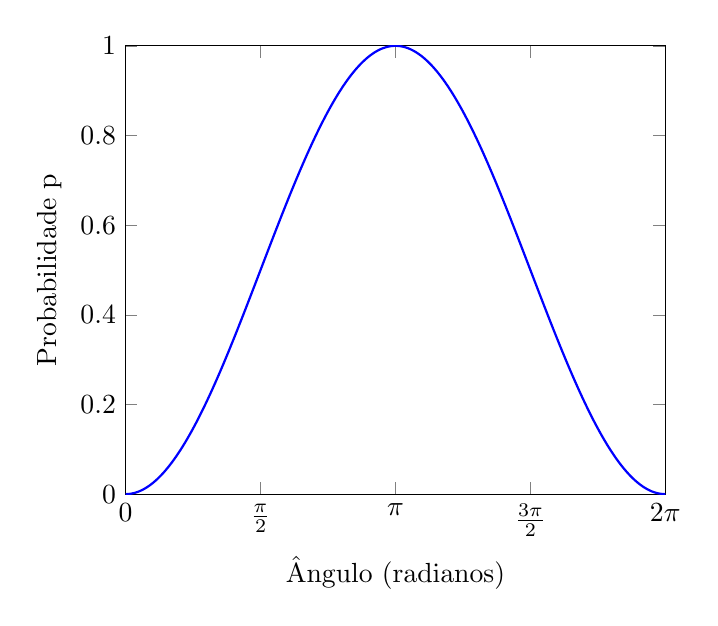
\begin{tikzpicture}
		\begin{axis}[
		xmin=0,xmax=2*pi,xlabel={Ângulo (radianos)},
		xtick={0, 1.5708, 3.14159, 4.7123889, 6.28318},
		xticklabels={$0$, $\frac{\pi}{2}$, $\pi$, $\frac{3\pi}{2}$, $2\pi$},
		ymin=0,ymax=1,ylabel={Probabilidade p}
		]
		\addplot[domain=0:2*pi,samples=200,smooth,thick,blue] {(sin(deg(x-pi/2))+1)/2};
		\end{axis}
		\end{tikzpicture}
		\caption{Gráfico da função $\left(\sin\left(x - \pi / 2\right) + 1\right) / 2$.}
		\label{graph:heap:request:alg}
	\end{figure}
	
	O algoritmo prossegue, então, da seguinte forma:
	
	\begin{enumerate}
		\item Obter um número $x$ pseudoaleatório no intervalo $[0, 2\pi]$;
		\item Calcular a probabilidade $p$ tal que $p = f(x) \times \SI{100}{\percent}$;
		\item Obter um número $r$ pseudoaleatório no intervalo $[0, 100]$;
		\item Caso $0 \leq r \leq p$, devolver 1. Se não, devolver 0.
	\end{enumerate}

	Isto traduz-se, portanto, no seguinte código em linguagem C:

	\begin{minted}[linenos]{c}
#define M_PI acos(-1.0)
int heaprequest(void) {
   double x = (rand() % 6284) / 1000.;
   int p = (int) ((sin(x - M_PI / 2.) + 1.) / 2. * 100.);
   int r = rand() % 101;
   return (p - r >= 0);
}
	\end{minted}
	
	Este algoritmo introduz, desta forma, 2 pontos de pseudo-aleatoriedade.
	
	
	\section{Relatório e estatísticas}
	\label{ssec:heap:stat}
	
	No final da execução do \chronOS~é impressa a estatística de utilização das 4 memórias \textit{heap} (Figura \ref{fig:heapreport}). Esta inclui as seguintes informações:
	
	\begin{itemize}
		\item \verb|Calls|: número total de solicitações de alocação;
		\item \verb|Crossed|: total de partições percorridas durante os processos de alocação;
		\item \verb|Leaks (KB)|: quantidade em KB de memória que não foram libertados pelos respetivos processos (\textit{memory leaks});
		\item \verb|# fragments|: quantidade de fragmentos externos com 1 ou 2 partições de tamanho;
		\item \verb|Alloc avg time|: tempo médio de alocação;
		\item \verb|Perc no-alloc|: percentagem de solicitações de alocação negadas.
	\end{itemize}
	
	Infelizmente, por motivos que não conseguimos até ao momento compreender, o programa contabiliza sempre que demorou 0 \textit{ticks} de \textit{clock} do programa para alocar a memória dinâmica, apesar de esta ser de facto alocada corretamente por cada um dos algoritmos. Testámos diferentes métodos sem sucesso. O que permaneceu no código final envolve a utilização do método \verb|clock()|. Várias referências na Internet argumentam fortemente contra o uso de alternativas como o \verb|gettimeofday()| para este fim, pelo que não os aplicámos.
	
	\begin{figure}[!htbp]
		\centering
		\includegraphics[width=\textwidth]{heapreport}
		\caption{Exemplo de um relatório das memórias dinâmicas.}
		\label{fig:heapreport}
	\end{figure}

	Para o modo de \textit{debug} é feita a impressão de um \textit{dump} das 4 memórias (exemplo na Figura \ref{fig:heapdump}). Tal permite verificar quais os processos que não libertaram os respetivos recursos alocados. Esta informação não é impressa em modo \textit{release} uma vez que pode ser bastante extensa e densa.
	
	\begin{figure}[!htbp]
		\centering
		\includegraphics[scale=0.6]{heapdump}
		\caption{Exemplo de um \textit{dump} de uma das memórias dinâmicas em modo \textit{debug}.}
		\label{fig:heapdump}
	\end{figure}

	
	\chapter{Leitura e execução de um programa}
	\label{sec:program}
	
	No \chronOS, um programa é um conjunto de \textbf{instruções} constituídas por 3 elementos: instrução, valor inteiro e nome de processo filho. A estrutura \verb|instruction| definida em \verb|types.h| define, portanto, uma instrução.
	
	O módulo \texttt{instructions} (definido com os respetivos \textit{header file} e ficheiro \verb|*.c|) contém as funções que executam as instruções propriamente ditas, conforme definidas em enunciado.
	
	O método \verb|program_read_from_file| lê as instruções de um programa, guardado num ficheiro com a extensão \verb|*.prg|, e aloca em memória \textit{heap} um vetor de instruções, cujo apontador é retornado como resultado.
	
	O método \verb|memalloc| recebe um vetor deste tipo e a sua dimensão, e assim aloca no bloco de memória \verb|memory| o espaço necessário para armazenar as instruções, fazendo uma cópia.
	
	O vetor alocado por \verb|program_read_from_file| não é libertado pelo método \verb|memalloc|, pelo que um \verb|free| deve ser executado após este último método.
	
	Os algoritmos de escalonamento são responsáveis por invocar o método \verb|run|, o qual executa a próxima instrução de um processo.
	
	
	\chapter{Discussão e conclusão}
	\label{sec:con_futwork}
	
	O projeto \chronOS~permitiu consolidar uma vasta gama de conhecimentos, não só de Sistemas Operativos como também de Estruturas de Dados e da linguagem C \textit{per se}.
	
	A forte estruturação do projeto em diferentes módulos, constituindo o que chamámos de \textit{Runtime Libraries Package} (RTL), permite que este seja facilmente escalável para mais algoritmos de escalonamento, além de ter facilitado a implementação de certas componentes do \textit{core} do programa.
	
	
	\section{Análise SWOT}
	
	Para discussão do projeto \chronOS, propomos a \textbf{análise SWOT} infra-apresentada.
	
	Os pontos fracos e respetivas oportunidades representam pontos potenciais para trabalho futuro.
	
	\subsection{Pontos fortes}
	
	\begin{enumerate}
		\item Código modular e facilmente escalável.
		\item Forte documentação do código.
		\item Criação de dois modos de compilação (\textit{debug} e \textit{release}).
		\item Implementação sólida do algoritmo \ac{FCFS}.
		\item Forte gestão de memória estática com recurso ao algoritmo \textit{first-fit}.
		\item Clara separação entre gestão de processos e gestão de memória.
		\item Implementação de uma \textit{queue} própria para gestão do plano de execução.
		\item Códigos compactos e objetivos para os processos de \textit{fork} e limpeza de processos.
		\item Utilização correta e consistente de listas ligadas para a construção das memórias dinâmicas.
		\item Algoritmo próprio de pseudo-aleatoriedade para solicitações de alocação com fundamento matemático.
		\item Correta alocação e dealocação de memória com recurso aos 4 algoritmos de gestão.
		\item Inexistência de \textit{memory leaks} na execução do \chronOS.
	\end{enumerate}
	
	
	\subsection{Pontos fracos}
	
	\begin{enumerate}
		\item Falta de variedade de algoritmos de escalonamento.
		\item Não utilização do ficheiro \verb|control.txt| para controlo fino do \chronOS.
		\item Utilização insuficiente dos argumentos passados pela \textit{shell} para controlo dos parâmetros do \chronOS.
		\item Inexistência de leitura de prioridades de processos a partir do ficheiro \verb|plan.txt|.
	\end{enumerate}
	
	
	\subsection{Oportunidades}
	
	\begin{enumerate}
		\item Implementação de novos algoritmos de escalonamento, tais como \ac{SJF}, \ac{EDF} e \textit{round-robin}.
		\item Introdução de controlo manual ou automatizado, passo-a-passo, da execução do \chronOS~segundo uma sequência de instruções de controlo.
		\item Maior controlo dos parâmetros internos do \chronOS~através de argumentos passados pela \textit{shell}.
		\item Implementação de uma \textit{queue} de prioridades para escalonamento dinâmico.
	\end{enumerate}
	
	
	\subsection{Ameaças}
	
	\begin{enumerate}
		\item Maior dificuldade de leitura do código devido à vasta documentação interna.
		\item Escassez de algoritmos de gestão de processos não permite uma comparação efetiva entre eles.
		\item Potencial ineficiência de utilização da memória estática devido às desvantagens do \textit{first-fit}.
		\item Utilização de código próprio para \textit{queues} e listas ligadas pode acarretar \textit{bugs} inesperados por não ser um código público devidamente escrutinado e de eficácia comprovada.
		\item Utilização de algoritmos próprios, não verificado por pares, acarreta desvantagens inerentes.
	\end{enumerate}
	
	
	\section{Conclusão}
	
	Os objetivos iniciais propostos foram cumpridos na sua quase totalidade com o projeto \chronOS. A gestão de processos e a gestão das memórias são operacionais e executam eficazmente as funções elementares.
	
	Apesar de uma pequena seleção de objetivos não ter sido plenamente alcançada, outros objetivos não inicialmente planeados foram alcançados em seu lugar. A forte modulação do código revelou-se uma mais-valia na construção da aplicação \chronOS~e, em particular, na hora do respetivo \textit{debugging}. De igual forma, foi possível construir vários elementos fundamentais com códigos relativamente simples e compactos devido à criação de funções altamente especializadas e independentes.
	
	A forte separação dos gestores de processos e de memória permitiram que não existissem erros e \textit{bugs} cruzados. Ou seja, um \textit{bug} no gestor de processos, por exemplo, não afeta a gestão das memórias.
	
	A expansão deste programa na sua versão atual para albergar novos algoritmos é, portanto, facilmente alcançável no que diz respeito à comunicação entre os vários componentes que constituem o \textit{core} do programa.
	
	Alcançar um código consistente e com a devida separação entre componentes foi uma consequência natural da nossa decisão em modular os referidos componentes do \textit{core} do \chronOS.
	
	Este é, pois, um projeto de elevado interesse para se dar a sua continuidade no futuro para aprofundamento de conhecimentos.
	
	
	\chapter*{Acrónimos}
	\addcontentsline{toc}{chapter}{Acrónimos}
    \label{sec:acron}
    
    \begin{acronym}[FCFS]
    	\acro{CPU}{\emph{Central Processing Unit}}
    	\acro{EDF}{\emph{Earliest deadline first}}
        \acro{FCFS}{\emph{First Come, First Serve}}
        \acro{GCC}{\emph{GNU C Compiler}}
        \acro{PID}{\emph{Process Identifier}}
        \acro{PCB}{\emph{Process Control Block}}
        \acro{SJF}{\emph{Shortest Job First}}
    \end{acronym}
	
\end{document}
